\section{Example}

Example of using table 
\begin{table}[htbp]
    \caption{Table captions should be placed above the
    tables.}\label{tab1}
    \begin{tabular}{|l|l|l|}
    \hline
    Heading level &  Example & Font size and style\\
    \hline
    Title (centered) &  {\Large\bfseries Lecture Notes} & 14 point, bold\\
    1st-level heading &  {\large\bfseries 1 Introduction} & 12 point, bold\\
    2nd-level heading & {\bfseries 2.1 Printing Area} & 10 point, bold\\
    3rd-level heading & {\bfseries Run-in Heading in Bold.} Text follows & 10 point, bold\\
    4th-level heading & {\itshape Lowest Level Heading.} Text follows & 10 point, italic\\
    \hline
    \end{tabular}
\end{table} 
\FloatBarrier

\begin{table}[htbp]
    \caption{Comparison between old and new Robot.}\label{tab2}
    \centering
    \begin{tabular}{|c|c|c|}
    \hline
    \rowcolor[HTML]{C0C0C0}
    \textbf{Parameter} &  \textbf{Old Robot} & \textbf{New Robot} \\
    \hline
        Dimension & 52x52x80 cm & 50x50x80 cm \\
        \hline
        Weight & 40 kg & 38 kg \\
        \hline
        Robot's Speed & 2.2 m/s & 3 m/s \\
        \hline
        Kicking Speed & 6 m/s & 10 m/s \\
        \hline
        Dribble's Speed & 1.8 m/s & 2.5 m/s \\
        \hline
        Camera & Omnidirectional Camera & Omnidirectional Camera, Depth Camera \\ 
        & & and Thermal Camera \\
        \hline
        MCU & Mini PC and STM32 & PLC, Mini PC, and STM32 \\
        \hline
        Supply & 36 Vdc Li-Ion Battery & 2 x 9 Ah Cordless Battery 20 VDC \\
    \hline
    \end{tabular}
\end{table} 
\FloatBarrier


Example of using figure 
\begin{figure}[htbp]
    \centering
    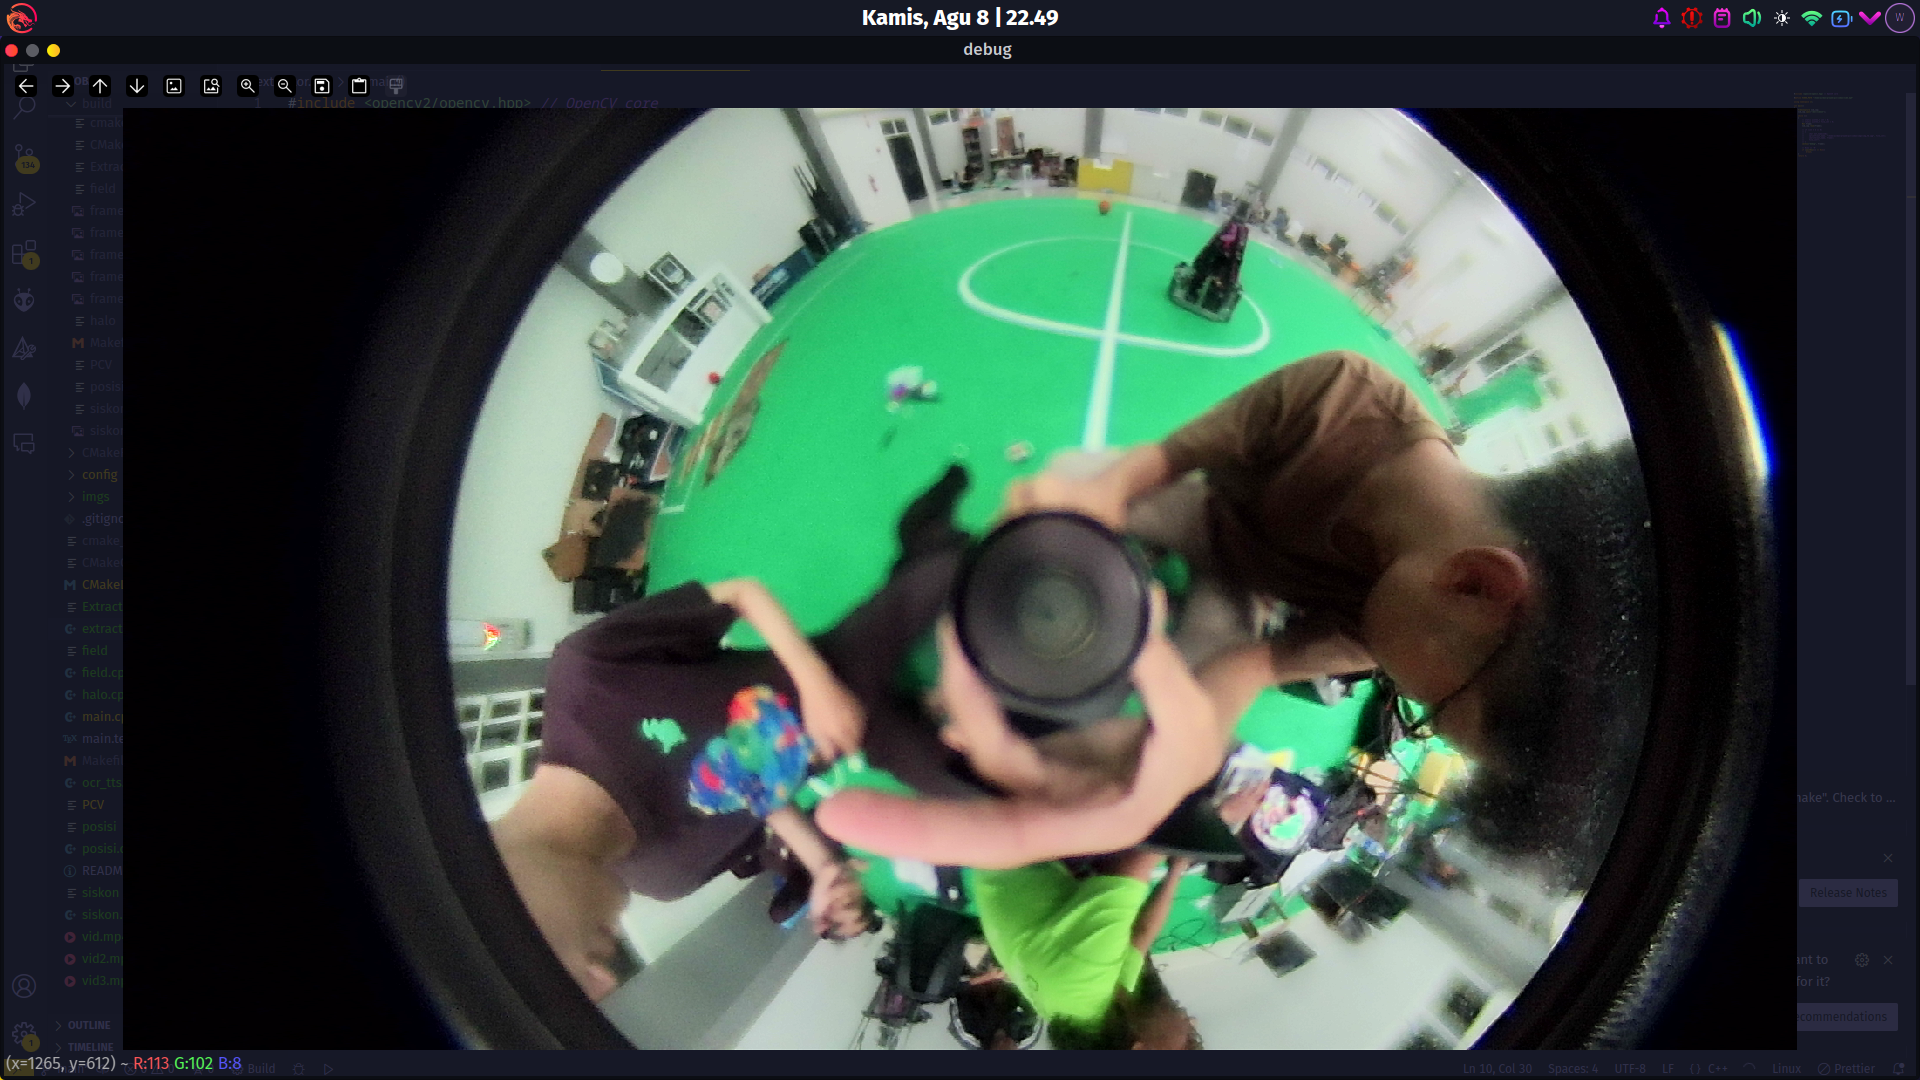
\includegraphics[width=\textwidth]{images/leopard3.png}
    \caption{A figure caption is always placed below the illustration.
    Please note that short captions are centered, while long ones are
    justified by the macro package automatically.} \label{fig1}
\end{figure}
\FloatBarrier

Example of using figure 2 
\begin{figure}[htbp]
    \centering
    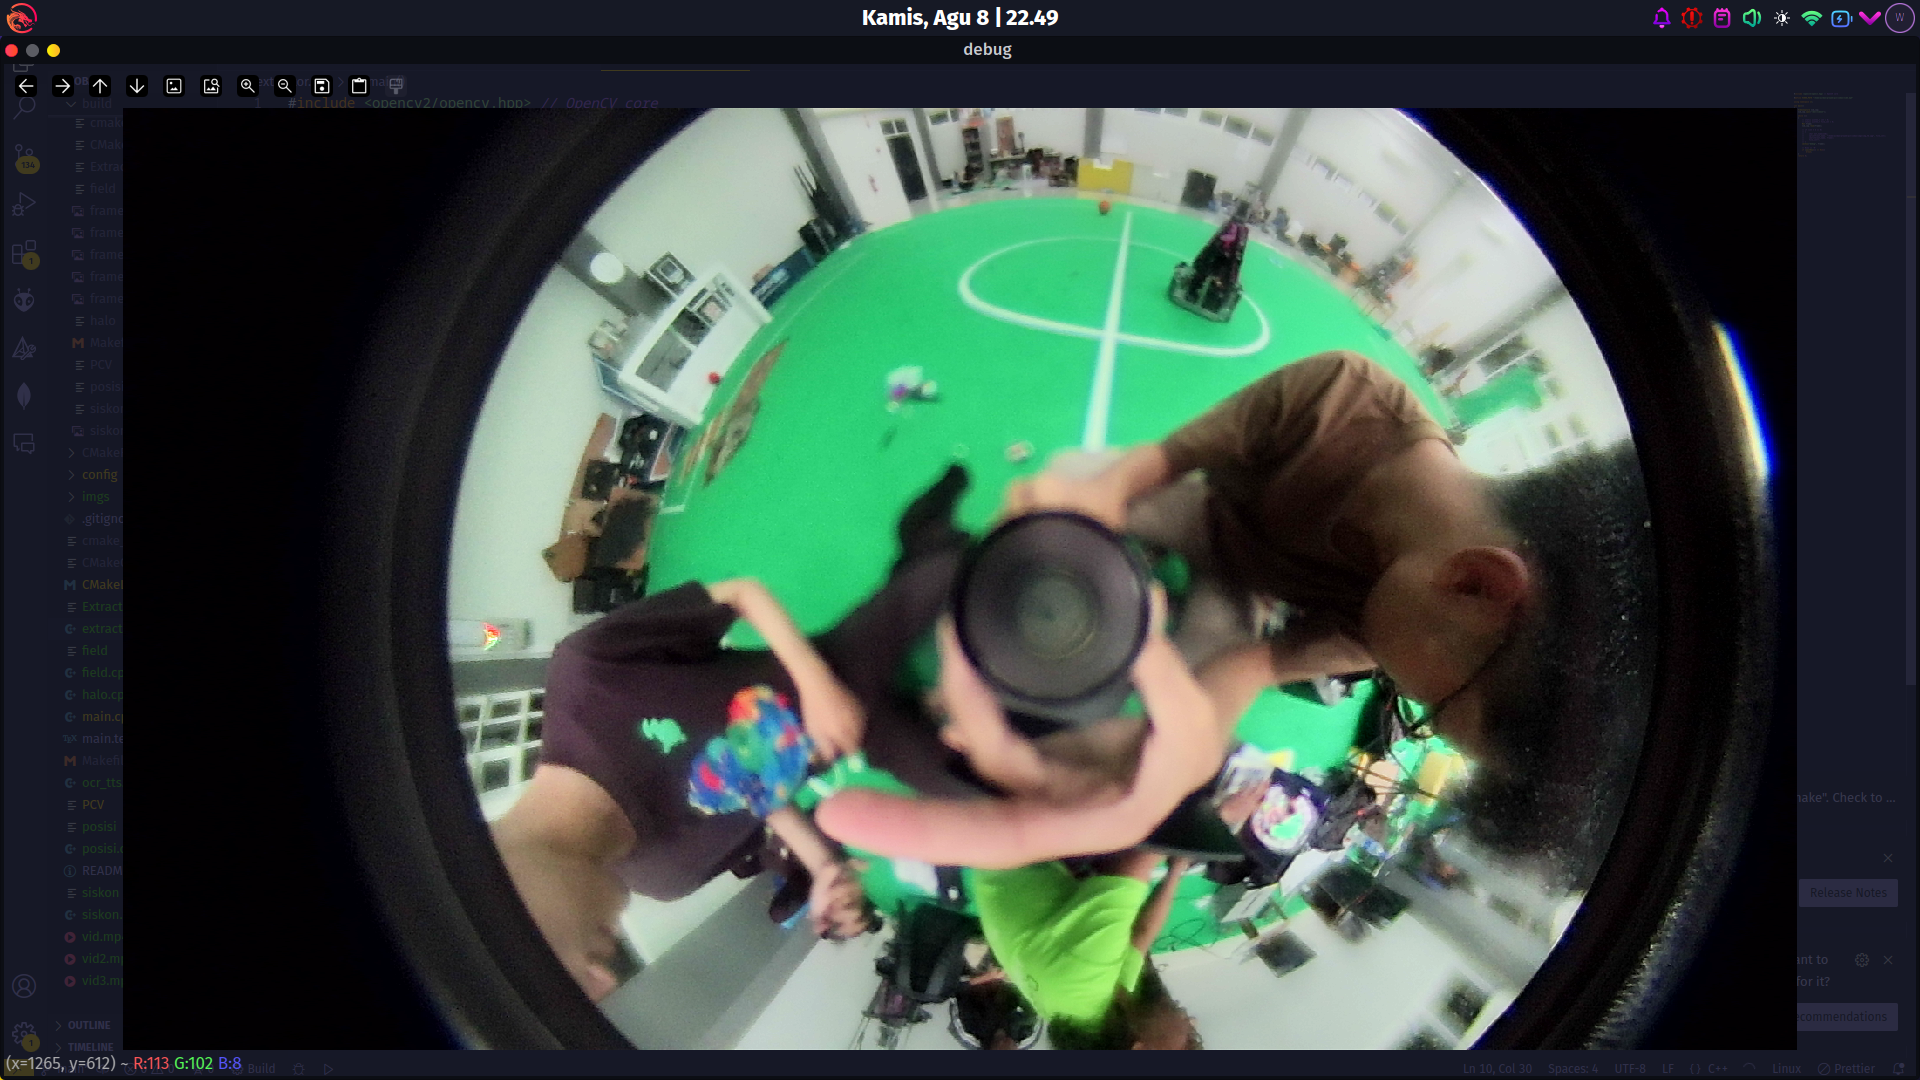
\includegraphics[width=4cm]{images/leopard3.png}
    \caption{A figure caption is always placed below the illustration.
    Please note that short captions are centered, while long ones are
    justified by the macro package automatically.} \label{fig2}
\end{figure}
\FloatBarrier

Example of using equation 
\begin{equation}
    x + y = z
\end{equation}

Example of using theorem
\begin{theorem}
    Theorem content, for example: $x + y = z$
\end{theorem}

Example of using proof
\begin{proof}
    Proof content, for example: $x + y = z$
\end{proof}

Example of using algorithm
\begin{algorithm}[H]
    \caption{Process Lines on Frame}\label{alg:process_lines}
    \begin{algorithmic}[1]
    \Procedure{ProcessLinesOnFrame}{}
        \State \text{Initialize lines\_on\_frame as an empty vector}
        \For{\text{angle from 0 to 360 with step size 2.5}}
            \State \text{Initialize dist to 0}
            \For{\text{index from 0 to 320}}
                \State $x \gets \text{dist} \times \cos(\text{angle}) + \text{center\_cam\_x}$
                \State $y \gets \text{center\_cam\_y} - \text{dist} \times \sin(\text{angle})$
                \If{\text{frame[y][x] == 255}}
                    \State \text{Push (x, y) to lines\_on\_frame}
                \EndIf
                \State $dist \gets \text{dist} + 1$
            \EndFor
        \EndFor
    \EndProcedure
    \end{algorithmic}
\end{algorithm}


Example of include program 
\lstinputlisting[
language=C++,
caption={Program test waktu.},
label={lst:test}
]{programs/time_test.cpp}

Example of include program 2
\lstinputlisting[
language=JavaScript,
caption={Program JavaScript.},
label={lst:testJS}
]{programs/something.js}


Example of using citation \cite{ref_url1}.